\section*{Введение}

В данной работе будет проведено полное исследование заданной функции, взятой из типового расчета по математике \cite{tip}: 
\begin{equation}
    \centering
    \label{eq:eq1}
    y = \frac{x^2-3}{x-2}.
\end{equation}

 Исследование функции будет проводиться по следующей схеме:
\begin{itemize}
    \item нахождение области значения функции;
    \item проверка на периодичность;
    \item исследование функции с помощью первой производной;
    \item исследование функции с помощью второй производной;
    \item проверка на наличие вертикальных, горизонтальных и наклонных асимптот графика функции;
    \item нахождение точек пересечения графика с координатными осями.
\end{itemize}

\addcontentsline{toc}{section}{Введение}

\newpage
\section{Исследование функции}

\subsection{Область определения функции}

Областью определения функции $\eqref{eq:eq1}$ является вся числовая ось, кроме точки $x = 2$.

\subsection{Проверка на периодичность}

Функция не является периодической. Проверим четность (нечетность):

\[f(-x) = \frac{(-x)^2-3}{-x-2} ;\ f(-x) = \frac{x^2-3}{-x-2} ;\ f(-x) \neq \frac{x^2-3}{x-2} ;\ f(-x) \neq -f(x).\]

Значит, функция не является ни чётной, ни нечётной. График функции не
имеет симметрии ни относительно оси ординат, ни относительно центра
системы координат.

\subsection{Исследование функции с помощью первой производной}

Найдём первую производную функции $\eqref{eq:eq1}$:

\[y' = \left(\frac{x^2-3}{x-2}\right)' = \frac{(x^2-3)'(x-2)-(x^2-3)(x-2)'}{(x-2)^2}  = \frac{x^2-4x+3}{(x-2)^2} = \frac{(x-1)(x-3)}{(x-2)^2}.\]

Тогда $y' = 0$ при $x_1 = 1, x_2 = 3$.

Проверим знаки производной и определим промежутки монотонности функции (рисунок \ref{pic:prom}). Таким образом, функция $\eqref{eq:eq1}$ возрастает при $x \in (-\infty;1) \cup (3; +\infty)$ и убывает при $x \in (1;2) \cup (2;3)$. Далее, так как при переходе через стационарную точку $x = 1$ производная меняет знак с плюса на минус, то $x=1$ точка максимума $(y_{max} = y(1) = 2)$. Аналогично, при переходе через стационарную точку
$x = 3$ производная меняет знак с минуса на плюс, поэтому $x = 3$ точка минимума $(y_{min} = y(3) = 6)$

\begin{figure}[H]
	\begin{center}
		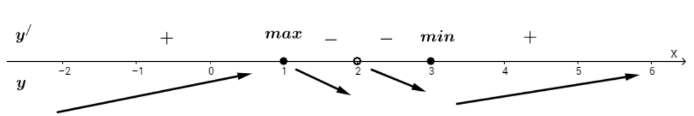
\includegraphics[scale=1]{prom}
		\caption{Промежутки монотонности функции $\eqref{eq:eq1}$}
		\label{pic:prom}
	\end{center}
\end{figure}

\subsection{Исследование функции с помощью второй производной}

Найдём вторую производную функции $\eqref{eq:eq1}$:

\[y'' = \left(\frac{x^2-3}{x-2}\right)'' = \left(\frac{x^2-4x+3}{(x-2)^2}\right)' = \frac{(2x-4)(x-2)^2 - (x^2-4x+3)2(x-2)}{(x-2)^4} = \frac{2}{(x-2)^3}.\]

Проверим знаки второй производной функции и определим промежутки выпуклости (вогнутости) функции (рисунок \ref{pic:vogn}).

\begin{figure}[H]
	\begin{center}
		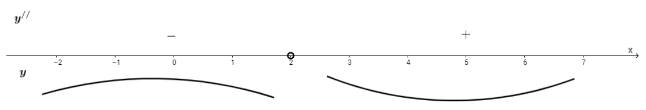
\includegraphics[scale=1.1]{vogn}
		\caption{Промежутки выпуклости (вогнутости) функции $\eqref{eq:eq1}$}
		\label{pic:vogn}
	\end{center}
\end{figure}

Таким образом, функция $\eqref{eq:eq1}$ выпукла вверх при $x \in (-\infty; 2)$ и выпукла вниз (вогнута) при $x \in (2; +\infty)$. Так как точка $x = 2$ не принадлежит области определения функции, она не является и точкой перегиба функции.

\subsection{Проверка на наличие асимптот}

Так как функция $\eqref{eq:eq1}$ не является непрерывной в точке $x = 2$, проверим в этой точке наличие вертикальной асимптоты:

Найдём $\lim\limits_{x\to 2-0} \frac{x^2-3}{x-2} = \frac{1}{-0} = -\infty, \lim\limits_{x\to 2+0} \frac{x^2-3}{x-2} = \frac{1}{+0} = +\infty$, откуда следует, что прямая $x = 2$ является вертикальной асимптотой.

Проверим наличие горизонтальной асимптоты $y = b$: $b = \lim\limits_{x\to \pm \infty} \frac{x^2-3}{x-2} =  \pm \infty \neq const$, откуда следует, что горизонтальной асимптоты нет.

Проверим наличие наклонной асимптоты $y = kx + b$: $k = \lim\limits_{x\to \pm \infty} \frac{f(x)}{x} = \lim\limits_{x\to \pm \infty} \frac{x^2-3}{x(x-2)} = 1,$ $b = \lim\limits_{x\to \pm \infty} f(x) - kx = \lim\limits_{x\to \pm \infty} \left(\frac{x^2-3}{(x-2)}-x\right) = \lim\limits_{x\to \pm \infty} \left(\frac{x^2-3-x(x-2)}{(x-2)}\right) = \lim\limits_{x\to \pm \infty}\left(\frac{2x-3}{x-2}\right) = 2.$

Значит, прямая $y = x + 2$ наклонная асимптота.

\subsection{Нахождение пересечений с осями координат}

Находим точки пересечения функции с координатными осями (таблица \ref{tabular:tab1}): 

\begin{table}[H]
	\caption{Пересечения функции с координатными осями}
	\begin{center}
		\begin{tabular}{|c|c|c|c|}
			\hline
			x & 0 & $\sqrt{3}$ & $-\sqrt{3}$ \\ \hline
			y & 1.5 & 0 & 0 \\ \hline
		\end{tabular}
		\label{tabular:tab1}
	\end{center}
\end{table}

Дополнительные точки: $y(4) = 6,5$; $y(-4) \approx -2,17.$


\section{Построение графика}
\subsection{Построение графика функции по заданию}

График функции представлен на рисунке \ref{pic:gr}:

\begin{figure}[H]
	\begin{center}
		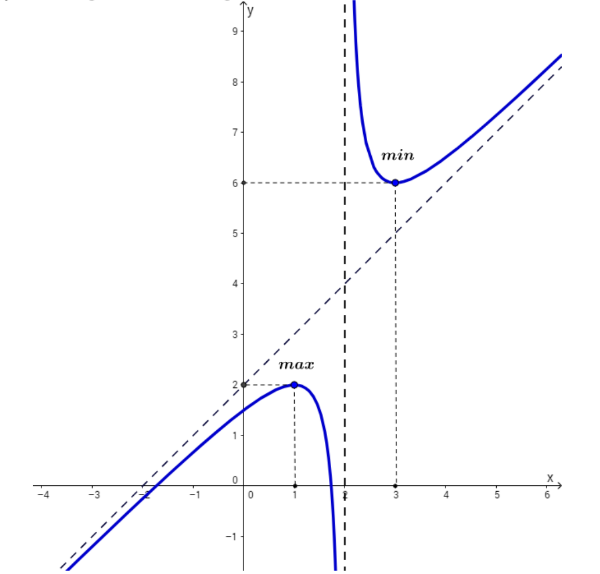
\includegraphics[scale=1]{gr}
		\caption{График функции $\eqref{eq:eq1}$}
		\label{pic:gr} 
	\end{center}
\end{figure}

\subsection{Проверка графика функции}

Проверим построенный график при помощи сайта \cite{desmos}. Введем функцию $\eqref{eq:eq1}$ и получим график, представленный на рисунке \ref{pic:des}:

\begin{figure}[H]
	\begin{center}
		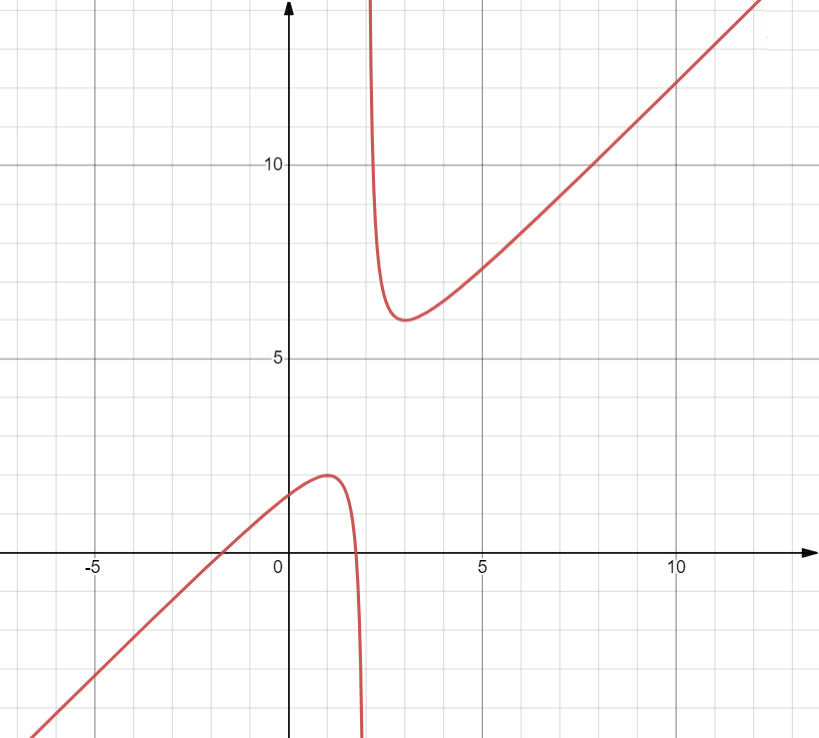
\includegraphics[scale=0.8]{des}
		\caption{График функции $\eqref{eq:eq1}$, построенный сайтом}
		\label{pic:des} 
	\end{center}
\end{figure}

Графики совпадают, следовательно, график функции $\eqref{eq:eq1}$ был построен верно.

\newpage
\section*{Заключение}
В данном типовом расчете была исследована функция $\eqref{eq:eq1}$, а также построен ее график.
\addcontentsline{toc}{section}{Заключение}